\begin{frame}{Gradient Boosting: what is it?}
	\begin{figure}
		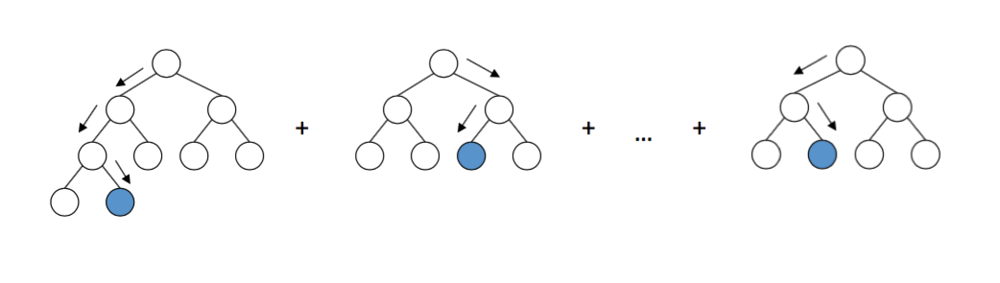
\includegraphics[width=\textwidth]{figures/gbdt}
	\end{figure}
\end{frame}

\begin{frame}{Gradient Boosting: libraries}
	\begin{columns}
		\begin{column}{0.33\textwidth}
			\centering
			\begin{figure}
				
\includegraphics[width=\columnwidth]{figures/scikit}
			\end{figure}
		\end{column}

		
		\begin{column}{0.33\textwidth}
			\centering
			\begin{figure}
				
\includegraphics[width=\columnwidth]{figures/catboost}
			\end{figure}
		\end{column}
		
		\begin{column}{0.33\textwidth}
			\centering
			\begin{figure}
				
\includegraphics[width=\columnwidth]{figures/xgboost}
			\end{figure}
		\end{column}
		
	\end{columns}
\end{frame}


\begin{frame}{Related work}
	\begin{enumerate}
		\item[\textbf{[1]}] Tianqi Chen and Carlos Guestrin. 2016. XGBoost: A Scalable Tree Boosting System. 
		\item[\textbf{[2]}] Anna Veronika Dorogush, Vasily Ershov, Andrey Gulin. 2017. CatBoost: gradient boosting with categorical features support
	\end{enumerate}
\end{frame}

\begin{frame}{Data}
	
\end{frame}
